\documentclass{whiteboard}
\begin{document}
\begin{frame}[plain,t]
\bbcover{Grafos}{Decteção de ciclos em grafos de sucessores}{Prof. Edson Alves}{Faculdade UnB Gama}

\end{frame}
\begin{frame}[plain,t]
\begin{tikzpicture}
\node[draw,opacity=0] at (0, 0) {x};
\node[draw,opacity=0] at (14, 8) {x};

	\node[anchor=west] (title) at (0.0, 6.5) { \Large \bbbold{Identificação de ciclos} };
\end{tikzpicture}
\end{frame}
\begin{frame}[plain,t]
\begin{tikzpicture}
\node[draw,opacity=0] at (0, 0) {x};
\node[draw,opacity=0] at (14, 8) {x};

	\node[anchor=west] (title) at (0.0, 6.5) { \Large \bbbold{Identificação de ciclos} };

	\node[anchor=west] (a) at (1.0, 5.5) { \bbtext{Seja $G$ um grafo de sucessores que contém um caminho que termine em} };

	\node[anchor=west] (a1) at (0.5, 4.75) { \bbtext{um ciclo.} };

\end{tikzpicture}
\end{frame}
\begin{frame}[plain,t]
\begin{tikzpicture}
\node[draw,opacity=0] at (0, 0) {x};
\node[draw,opacity=0] at (14, 8) {x};

	\node[anchor=west] (title) at (0.0, 6.5) { \Large \bbbold{Identificação de ciclos} };

	\node[anchor=west] (a) at (1.0, 5.5) { \bbtext{Seja $G$ um grafo de sucessores que contém um caminho que termine em} };

	\node[anchor=west] (a1) at (0.5, 4.75) { \bbtext{um ciclo.} };


	\node[anchor=west] (b) at (1.5, 4.0) { \bbtext{$1$. Qual é o nó de menor índice que pertence ao ciclo? $(\mu)$} };

	\node[anchor=west] (b1) at (1.5, 3.5) { \bbtext{$2$. O ciclo contém quantos nós? $(\lambda)$} };

\end{tikzpicture}
\end{frame}
\begin{frame}[plain,t]
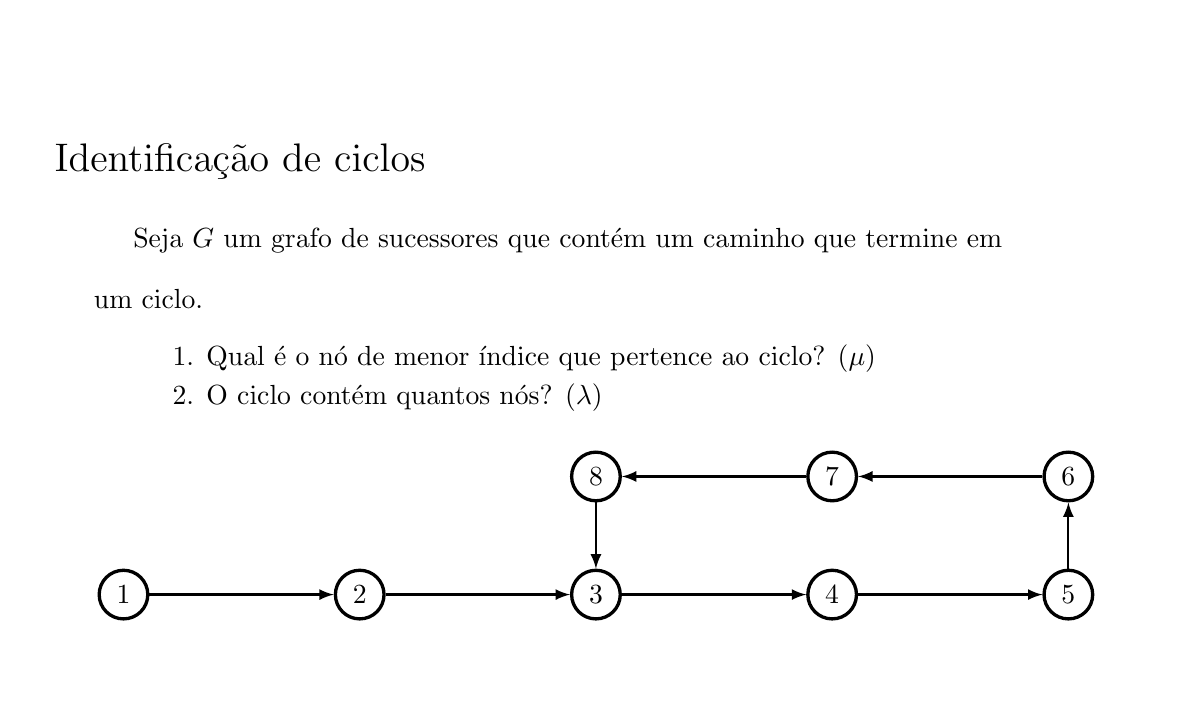
\begin{tikzpicture}
\node[draw,opacity=0] at (0, 0) {x};
\node[draw,opacity=0] at (14, 8) {x};

	\node[anchor=west] (title) at (0.0, 6.5) { \Large \bbbold{Identificação de ciclos} };

	\node[anchor=west] (a) at (1.0, 5.5) { \bbtext{Seja $G$ um grafo de sucessores que contém um caminho que termine em} };

	\node[anchor=west] (a1) at (0.5, 4.75) { \bbtext{um ciclo.} };


	\node[anchor=west] (b) at (1.5, 4.0) { \bbtext{$1$. Qual é o nó de menor índice que pertence ao ciclo? $(\mu)$} };

	\node[anchor=west] (b1) at (1.5, 3.5) { \bbtext{$2$. O ciclo contém quantos nós? $(\lambda)$} };


	\node[very thick,draw,circle] (node1) at (1.0, 1.0) { \bbtext{1} };

	\node[very thick,draw,circle] (node2) at (4.0, 1.0) { \bbtext{2} };

	\node[very thick,draw,circle] (node3) at (7.0, 1.0) { \bbtext{3} };

	\node[very thick,draw,circle] (node4) at (10.0, 1.0) { \bbtext{4} };

	\node[very thick,draw,circle] (node5) at (13.0, 1.0) { \bbtext{5} };

	\node[very thick,draw,circle] (node6) at (13.0, 2.5) { \bbtext{6} };

	\node[very thick,draw,circle] (node7) at (10.0, 2.5) { \bbtext{7} };

	\node[very thick,draw,circle] (node8) at (7.0, 2.5) { \bbtext{8} };

	\draw[thick,-latex](node1) to (node2);

	\draw[thick,-latex](node2) to (node3);

	\draw[thick,-latex](node3) to (node4);

	\draw[thick,-latex](node4) to (node5);

	\draw[thick,-latex](node5) to (node6);

	\draw[thick,-latex](node6) to (node7);

	\draw[thick,-latex](node7) to (node8);

	\draw[thick,-latex](node8) to (node3);


\end{tikzpicture}
\end{frame}
\begin{frame}[plain,t]
\begin{tikzpicture}
\node[draw,opacity=0] at (0, 0) {x};
\node[draw,opacity=0] at (14, 8) {x};

	\node[anchor=west] (title) at (0.0, 6.5) { \Large \bbbold{Algoritmo linear em execução e memória} };
\end{tikzpicture}
\end{frame}
\begin{frame}[plain,t]
\begin{tikzpicture}
\node[draw,opacity=0] at (0, 0) {x};
\node[draw,opacity=0] at (14, 8) {x};

	\node[anchor=west] (title) at (0.0, 6.5) { \Large \bbbold{Algoritmo linear em execução e memória} };

	\node[anchor=west] (a) at (1.0, 5.5) { \bbtext{$1$. Faça $u = 1$ e $s = \emptyset$} };

\end{tikzpicture}
\end{frame}
\begin{frame}[plain,t]
\begin{tikzpicture}
\node[draw,opacity=0] at (0, 0) {x};
\node[draw,opacity=0] at (14, 8) {x};

	\node[anchor=west] (title) at (0.0, 6.5) { \Large \bbbold{Algoritmo linear em execução e memória} };

	\node[anchor=west] (a) at (1.0, 5.5) { \bbtext{$1$. Faça $u = 1$ e $s = \emptyset$} };


	\node[anchor=west] (b) at (1.0, 4.5) { \bbtext{$2$. Enquanto $u\not\in s$:} };

\end{tikzpicture}
\end{frame}
\begin{frame}[plain,t]
\begin{tikzpicture}
\node[draw,opacity=0] at (0, 0) {x};
\node[draw,opacity=0] at (14, 8) {x};

	\node[anchor=west] (title) at (0.0, 6.5) { \Large \bbbold{Algoritmo linear em execução e memória} };

	\node[anchor=west] (a) at (1.0, 5.5) { \bbtext{$1$. Faça $u = 1$ e $s = \emptyset$} };


	\node[anchor=west] (b) at (1.0, 4.5) { \bbtext{$2$. Enquanto $u\not\in s$:} };


	\node[anchor=west] (b1) at (1.5, 3.75) { \bbtext{$(a)$ Insira $u$ em $s$} };

\end{tikzpicture}
\end{frame}
\begin{frame}[plain,t]
\begin{tikzpicture}
\node[draw,opacity=0] at (0, 0) {x};
\node[draw,opacity=0] at (14, 8) {x};

	\node[anchor=west] (title) at (0.0, 6.5) { \Large \bbbold{Algoritmo linear em execução e memória} };

	\node[anchor=west] (a) at (1.0, 5.5) { \bbtext{$1$. Faça $u = 1$ e $s = \emptyset$} };


	\node[anchor=west] (b) at (1.0, 4.5) { \bbtext{$2$. Enquanto $u\not\in s$:} };


	\node[anchor=west] (b1) at (1.5, 3.75) { \bbtext{$(a)$ Insira $u$ em $s$} };


	\node[anchor=west] (b2) at (1.5, 3.0) { \bbtext{$(b)$ Faça $u = \mathrm{succ}(u)$} };

\end{tikzpicture}
\end{frame}
\begin{frame}[plain,t]
\begin{tikzpicture}
\node[draw,opacity=0] at (0, 0) {x};
\node[draw,opacity=0] at (14, 8) {x};

	\node[anchor=west] (title) at (0.0, 6.5) { \Large \bbbold{Algoritmo linear em execução e memória} };

	\node[anchor=west] (a) at (1.0, 5.5) { \bbtext{$1$. Faça $u = 1$ e $s = \emptyset$} };


	\node[anchor=west] (b) at (1.0, 4.5) { \bbtext{$2$. Enquanto $u\not\in s$:} };


	\node[anchor=west] (b1) at (1.5, 3.75) { \bbtext{$(a)$ Insira $u$ em $s$} };


	\node[anchor=west] (b2) at (1.5, 3.0) { \bbtext{$(b)$ Faça $u = \mathrm{succ}(u)$} };


	\node[anchor=west] (c) at (1.0, 2.0) { \bbtext{$3$. $\mu = u$} };

\end{tikzpicture}
\end{frame}
\begin{frame}[plain,t]
\begin{tikzpicture}
\node[draw,opacity=0] at (0, 0) {x};
\node[draw,opacity=0] at (14, 8) {x};

	\node[anchor=west] (title) at (0.0, 6.5) { \Large \bbbold{Algoritmo linear em execução e memória} };

	\node[anchor=west] (a) at (1.0, 5.5) { \bbtext{$1$. Faça $u = 1$ e $s = \emptyset$} };


	\node[anchor=west] (b) at (1.0, 4.5) { \bbtext{$2$. Enquanto $u\not\in s$:} };


	\node[anchor=west] (b1) at (1.5, 3.75) { \bbtext{$(a)$ Insira $u$ em $s$} };


	\node[anchor=west] (b2) at (1.5, 3.0) { \bbtext{$(b)$ Faça $u = \mathrm{succ}(u)$} };


	\node[anchor=west] (c) at (1.0, 2.0) { \bbtext{$3$. $\mu = u$} };


	\node[anchor=west] (d) at (1.0, 1.0) { \bbtext{$4$. $\lambda = N - \mu + 1$, onde $N = |V|$} };

\end{tikzpicture}
\end{frame}
\begin{frame}[plain,t]

\inputsnippet{cpp}{5}{20}{codes/linear.cpp}

\end{frame}
\begin{frame}[plain,t]
\begin{tikzpicture}
\node[draw,opacity=0] at (0, 0) {x};
\node[draw,opacity=0] at (14, 8) {x};

	\node[anchor=west] (title) at (0.0, 6.0) { \Large \bbbold{Algoritmo de Floyd} };
\end{tikzpicture}
\end{frame}
\begin{frame}[plain,t]
\begin{tikzpicture}
\node[draw,opacity=0] at (0, 0) {x};
\node[draw,opacity=0] at (14, 8) {x};

	\node[anchor=west] (title) at (0.0, 6.0) { \Large \bbbold{Algoritmo de Floyd} };

	\node[anchor=west] (a) at (1.0, 5.0) { $\star$ \bbtext{Também conhecido como algoritmo da lebre e da tartaruga} };
\end{tikzpicture}
\end{frame}
\begin{frame}[plain,t]
\begin{tikzpicture}
\node[draw,opacity=0] at (0, 0) {x};
\node[draw,opacity=0] at (14, 8) {x};

	\node[anchor=west] (title) at (0.0, 6.0) { \Large \bbbold{Algoritmo de Floyd} };

	\node[anchor=west] (a) at (1.0, 5.0) { $\star$ \bbtext{Também conhecido como algoritmo da lebre e da tartaruga} };

	\node[anchor=west] (b) at (1.0, 4.0) { $\star$ \bbtext{Identifica um ciclo com execução $O(N)$ e memória $O(1)$} };
\end{tikzpicture}
\end{frame}
\begin{frame}[plain,t]
\begin{tikzpicture}
\node[draw,opacity=0] at (0, 0) {x};
\node[draw,opacity=0] at (14, 8) {x};

	\node[anchor=west] (title) at (0.0, 6.0) { \Large \bbbold{Algoritmo de Floyd} };

	\node[anchor=west] (a) at (1.0, 5.0) { $\star$ \bbtext{Também conhecido como algoritmo da lebre e da tartaruga} };

	\node[anchor=west] (b) at (1.0, 4.0) { $\star$ \bbtext{Identifica um ciclo com execução $O(N)$ e memória $O(1)$} };

	\node[anchor=west] (c) at (1.0, 3.0) { $\star$ \bbtext{Utilizada dois ponteiros: a lebre e a tartaruga} };
\end{tikzpicture}
\end{frame}
\begin{frame}[plain,t]
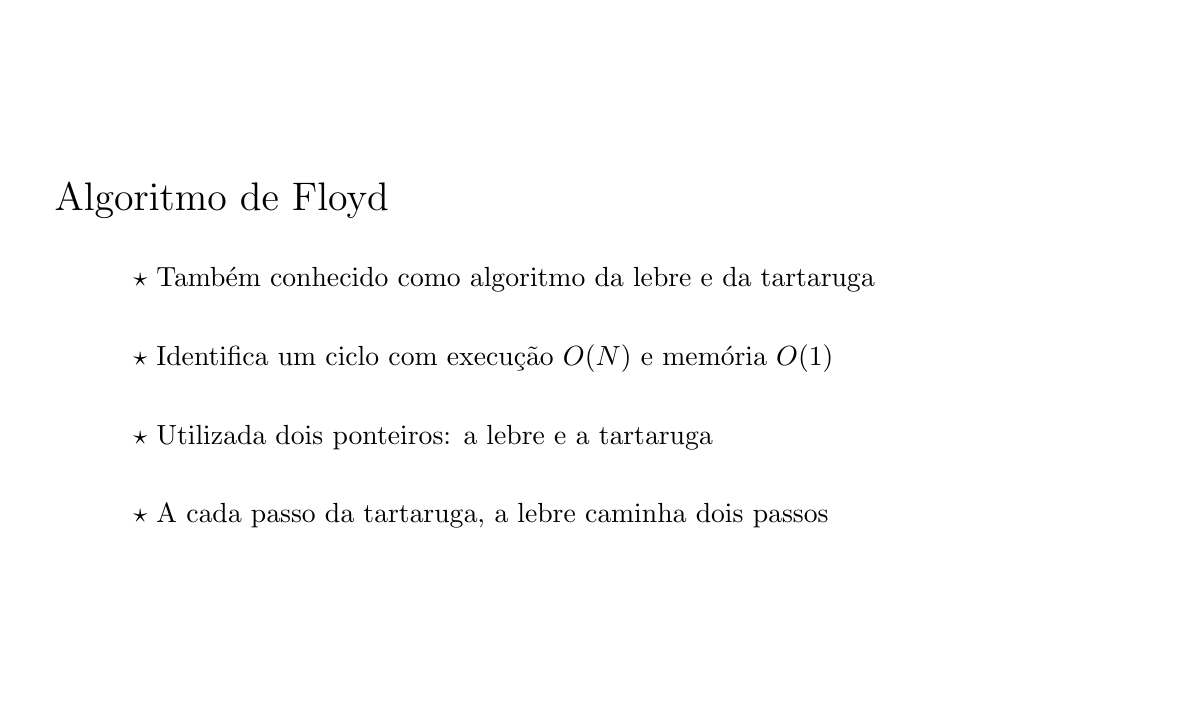
\begin{tikzpicture}
\node[draw,opacity=0] at (0, 0) {x};
\node[draw,opacity=0] at (14, 8) {x};

	\node[anchor=west] (title) at (0.0, 6.0) { \Large \bbbold{Algoritmo de Floyd} };

	\node[anchor=west] (a) at (1.0, 5.0) { $\star$ \bbtext{Também conhecido como algoritmo da lebre e da tartaruga} };

	\node[anchor=west] (b) at (1.0, 4.0) { $\star$ \bbtext{Identifica um ciclo com execução $O(N)$ e memória $O(1)$} };

	\node[anchor=west] (c) at (1.0, 3.0) { $\star$ \bbtext{Utilizada dois ponteiros: a lebre e a tartaruga} };

	\node[anchor=west] (d) at (1.0, 2.0) { $\star$ \bbtext{A cada passo da tartaruga, a lebre caminha dois passos} };
\end{tikzpicture}
\end{frame}
\begin{frame}[plain,t]
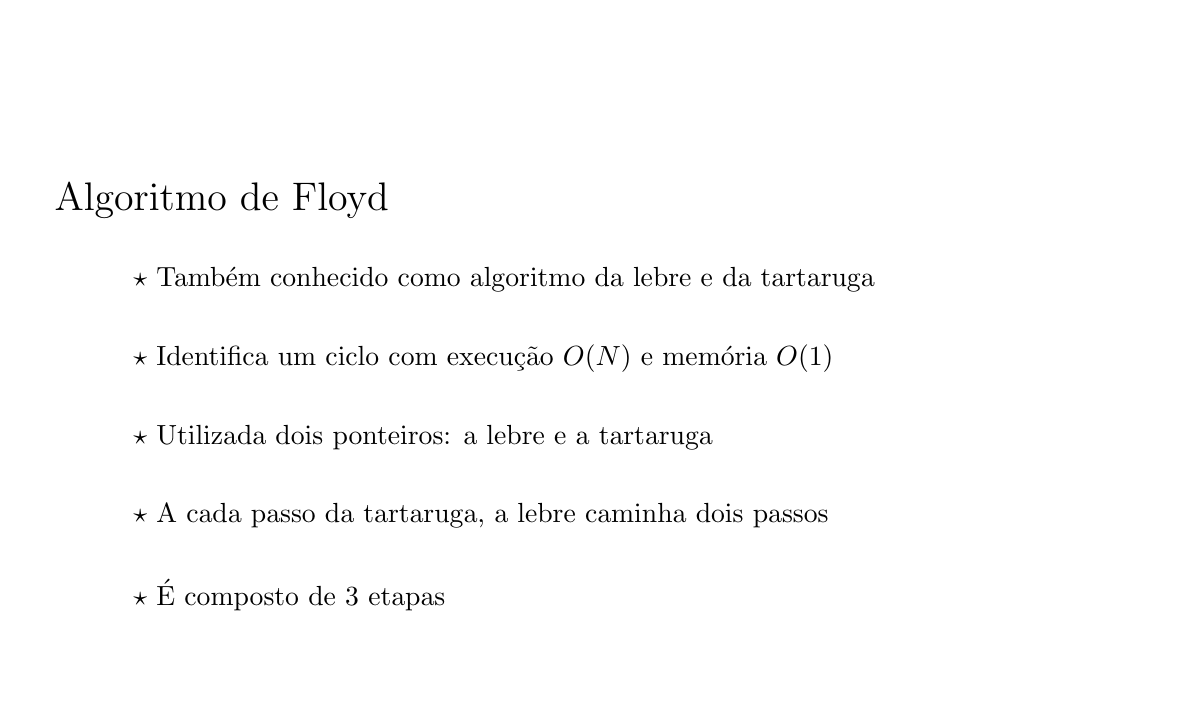
\begin{tikzpicture}
\node[draw,opacity=0] at (0, 0) {x};
\node[draw,opacity=0] at (14, 8) {x};

	\node[anchor=west] (title) at (0.0, 6.0) { \Large \bbbold{Algoritmo de Floyd} };

	\node[anchor=west] (a) at (1.0, 5.0) { $\star$ \bbtext{Também conhecido como algoritmo da lebre e da tartaruga} };

	\node[anchor=west] (b) at (1.0, 4.0) { $\star$ \bbtext{Identifica um ciclo com execução $O(N)$ e memória $O(1)$} };

	\node[anchor=west] (c) at (1.0, 3.0) { $\star$ \bbtext{Utilizada dois ponteiros: a lebre e a tartaruga} };

	\node[anchor=west] (d) at (1.0, 2.0) { $\star$ \bbtext{A cada passo da tartaruga, a lebre caminha dois passos} };

	\node[anchor=west] (e) at (1.0, 1.0) { $\star$ \bbtext{É composto de 3 etapas} };

\end{tikzpicture}
\end{frame}
\begin{frame}[plain,t]
\begin{tikzpicture}
\node[draw,opacity=0] at (0, 0) {x};
\node[draw,opacity=0] at (14, 8) {x};

	\node[anchor=west] (title) at (0.0, 6.5) { \Large \bbbold{Etapa 1: Identificação do ciclo} };
\end{tikzpicture}
\end{frame}
\begin{frame}[plain,t]
\begin{tikzpicture}
\node[draw,opacity=0] at (0, 0) {x};
\node[draw,opacity=0] at (14, 8) {x};

	\node[anchor=west] (title) at (0.0, 6.5) { \Large \bbbold{Etapa 1: Identificação do ciclo} };

	\node[very thick,draw,circle] (node1) at (1.0, 2.0) { \bbtext{1} };

	\node[very thick,draw,circle] (node2) at (4.0, 2.0) { \bbtext{2} };

	\node[very thick,draw,circle] (node3) at (7.0, 2.0) { \bbtext{3} };

	\node[very thick,draw,circle] (node4) at (10.0, 2.0) { \bbtext{4} };

	\node[very thick,draw,circle] (node5) at (13.0, 2.0) { \bbtext{5} };

	\node[very thick,draw,circle] (node6) at (13.0, 4.0) { \bbtext{6} };

	\node[very thick,draw,circle] (node7) at (10.0, 4.0) { \bbtext{7} };

	\node[very thick,draw,circle] (node8) at (7.0, 4.0) { \bbtext{8} };

	\draw[thick,-latex](node1) to (node2);

	\draw[thick,-latex](node2) to (node3);

	\draw[thick,-latex](node3) to (node4);

	\draw[thick,-latex](node4) to (node5);

	\draw[thick,-latex](node5) to (node6);

	\draw[thick,-latex](node6) to (node7);

	\draw[thick,-latex](node7) to (node8);

	\draw[thick,-latex](node8) to (node3);

\end{tikzpicture}
\end{frame}
\begin{frame}[plain,t]
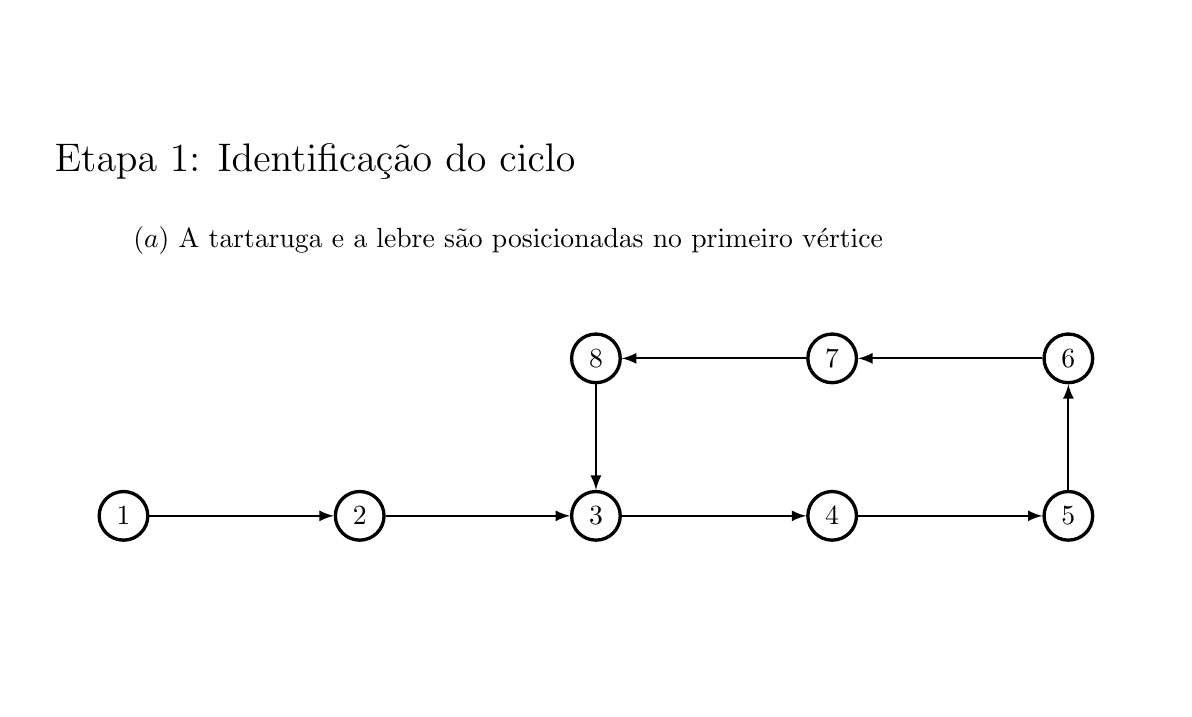
\begin{tikzpicture}
\node[draw,opacity=0] at (0, 0) {x};
\node[draw,opacity=0] at (14, 8) {x};

	\node[anchor=west] (title) at (0.0, 6.5) { \Large \bbbold{Etapa 1: Identificação do ciclo} };

	\node[very thick,draw,circle] (node1) at (1.0, 2.0) { \bbtext{1} };

	\node[very thick,draw,circle] (node2) at (4.0, 2.0) { \bbtext{2} };

	\node[very thick,draw,circle] (node3) at (7.0, 2.0) { \bbtext{3} };

	\node[very thick,draw,circle] (node4) at (10.0, 2.0) { \bbtext{4} };

	\node[very thick,draw,circle] (node5) at (13.0, 2.0) { \bbtext{5} };

	\node[very thick,draw,circle] (node6) at (13.0, 4.0) { \bbtext{6} };

	\node[very thick,draw,circle] (node7) at (10.0, 4.0) { \bbtext{7} };

	\node[very thick,draw,circle] (node8) at (7.0, 4.0) { \bbtext{8} };

	\draw[thick,-latex](node1) to (node2);

	\draw[thick,-latex](node2) to (node3);

	\draw[thick,-latex](node3) to (node4);

	\draw[thick,-latex](node4) to (node5);

	\draw[thick,-latex](node5) to (node6);

	\draw[thick,-latex](node6) to (node7);

	\draw[thick,-latex](node7) to (node8);

	\draw[thick,-latex](node8) to (node3);


	\node[anchor=west] (info) at (1.0, 5.5) { \bbtext{$(a)$ A tartaruga e a lebre são posicionadas no primeiro vértice} };

\end{tikzpicture}
\end{frame}
\begin{frame}[plain,t]
\begin{tikzpicture}
\node[draw,opacity=0] at (0, 0) {x};
\node[draw,opacity=0] at (14, 8) {x};

	\node[anchor=west] (title) at (0.0, 6.5) { \Large \bbbold{Etapa 1: Identificação do ciclo} };

	\node[very thick,draw,circle] (node1) at (1.0, 2.0) { \bbtext{1} };

	\node[very thick,draw,circle] (node2) at (4.0, 2.0) { \bbtext{2} };

	\node[very thick,draw,circle] (node3) at (7.0, 2.0) { \bbtext{3} };

	\node[very thick,draw,circle] (node4) at (10.0, 2.0) { \bbtext{4} };

	\node[very thick,draw,circle] (node5) at (13.0, 2.0) { \bbtext{5} };

	\node[very thick,draw,circle] (node6) at (13.0, 4.0) { \bbtext{6} };

	\node[very thick,draw,circle] (node7) at (10.0, 4.0) { \bbtext{7} };

	\node[very thick,draw,circle] (node8) at (7.0, 4.0) { \bbtext{8} };

	\draw[thick,-latex](node1) to (node2);

	\draw[thick,-latex](node2) to (node3);

	\draw[thick,-latex](node3) to (node4);

	\draw[thick,-latex](node4) to (node5);

	\draw[thick,-latex](node5) to (node6);

	\draw[thick,-latex](node6) to (node7);

	\draw[thick,-latex](node7) to (node8);

	\draw[thick,-latex](node8) to (node3);


	\node[anchor=west] (info) at (1.0, 5.5) { \bbtext{$(a)$ A tartaruga e a lebre são posicionadas no primeiro vértice} };


	\node[] (T) at (1.0, 1.25) { \includegraphics[scale=0.05]{figs/tortoise.png} };

	\node[] (H) at (1.0, 3.0) { \includegraphics[scale=0.03]{figs/rabbit.png} };

\end{tikzpicture}
\end{frame}
\begin{frame}[plain,t]
\begin{tikzpicture}
\node[draw,opacity=0] at (0, 0) {x};
\node[draw,opacity=0] at (14, 8) {x};

	\node[anchor=west] (title) at (0.0, 6.5) { \Large \bbbold{Etapa 1: Identificação do ciclo} };

	\node[very thick,draw,circle] (node1) at (1.0, 2.0) { \bbtext{1} };

	\node[very thick,draw,circle] (node2) at (4.0, 2.0) { \bbtext{2} };

	\node[very thick,draw,circle] (node3) at (7.0, 2.0) { \bbtext{3} };

	\node[very thick,draw,circle] (node4) at (10.0, 2.0) { \bbtext{4} };

	\node[very thick,draw,circle] (node5) at (13.0, 2.0) { \bbtext{5} };

	\node[very thick,draw,circle] (node6) at (13.0, 4.0) { \bbtext{6} };

	\node[very thick,draw,circle] (node7) at (10.0, 4.0) { \bbtext{7} };

	\node[very thick,draw,circle] (node8) at (7.0, 4.0) { \bbtext{8} };

	\draw[thick,-latex](node1) to (node2);

	\draw[thick,-latex](node2) to (node3);

	\draw[thick,-latex](node3) to (node4);

	\draw[thick,-latex](node4) to (node5);

	\draw[thick,-latex](node5) to (node6);

	\draw[thick,-latex](node6) to (node7);

	\draw[thick,-latex](node7) to (node8);

	\draw[thick,-latex](node8) to (node3);


	\node[anchor=west] (info) at (1.0, 5.5) { \bbtext{$(b)$ A lebre dá dois passos, a tartaruga um, até se reencontrarem} };


	\node[] (T) at (1.0, 1.25) { \includegraphics[scale=0.05]{figs/tortoise.png} };

	\node[] (H) at (1.0, 3.0) { \includegraphics[scale=0.03]{figs/rabbit.png} };


\end{tikzpicture}
\end{frame}
\begin{frame}[plain,t]
\begin{tikzpicture}
\node[draw,opacity=0] at (0, 0) {x};
\node[draw,opacity=0] at (14, 8) {x};

	\node[anchor=west] (title) at (0.0, 6.5) { \Large \bbbold{Etapa 1: Identificação do ciclo} };

	\node[very thick,draw,circle] (node1) at (1.0, 2.0) { \bbtext{1} };

	\node[very thick,draw,circle] (node2) at (4.0, 2.0) { \bbtext{2} };

	\node[very thick,draw,circle] (node3) at (7.0, 2.0) { \bbtext{3} };

	\node[very thick,draw,circle] (node4) at (10.0, 2.0) { \bbtext{4} };

	\node[very thick,draw,circle] (node5) at (13.0, 2.0) { \bbtext{5} };

	\node[very thick,draw,circle] (node6) at (13.0, 4.0) { \bbtext{6} };

	\node[very thick,draw,circle] (node7) at (10.0, 4.0) { \bbtext{7} };

	\node[very thick,draw,circle] (node8) at (7.0, 4.0) { \bbtext{8} };

	\draw[thick,-latex](node1) to (node2);

	\draw[thick,-latex](node2) to (node3);

	\draw[thick,-latex](node3) to (node4);

	\draw[thick,-latex](node4) to (node5);

	\draw[thick,-latex](node5) to (node6);

	\draw[thick,-latex](node6) to (node7);

	\draw[thick,-latex](node7) to (node8);

	\draw[thick,-latex](node8) to (node3);


	\node[anchor=west] (info) at (1.0, 5.5) { \bbtext{$(b)$ A lebre dá dois passos, a tartaruga um, até se reencontrarem} };


	\node[] (T) at (4.0, 1.25) { \includegraphics[scale=0.05]{figs/tortoise.png} };

	\node[] (H) at (7.0, 1.25) { \includegraphics[scale=0.03]{figs/rabbit.png} };




\end{tikzpicture}
\end{frame}
\begin{frame}[plain,t]
\begin{tikzpicture}
\node[draw,opacity=0] at (0, 0) {x};
\node[draw,opacity=0] at (14, 8) {x};

	\node[anchor=west] (title) at (0.0, 6.5) { \Large \bbbold{Etapa 1: Identificação do ciclo} };

	\node[very thick,draw,circle] (node1) at (1.0, 2.0) { \bbtext{1} };

	\node[very thick,draw,circle] (node2) at (4.0, 2.0) { \bbtext{2} };

	\node[very thick,draw,circle] (node3) at (7.0, 2.0) { \bbtext{3} };

	\node[very thick,draw,circle] (node4) at (10.0, 2.0) { \bbtext{4} };

	\node[very thick,draw,circle] (node5) at (13.0, 2.0) { \bbtext{5} };

	\node[very thick,draw,circle] (node6) at (13.0, 4.0) { \bbtext{6} };

	\node[very thick,draw,circle] (node7) at (10.0, 4.0) { \bbtext{7} };

	\node[very thick,draw,circle] (node8) at (7.0, 4.0) { \bbtext{8} };

	\draw[thick,-latex](node1) to (node2);

	\draw[thick,-latex](node2) to (node3);

	\draw[thick,-latex](node3) to (node4);

	\draw[thick,-latex](node4) to (node5);

	\draw[thick,-latex](node5) to (node6);

	\draw[thick,-latex](node6) to (node7);

	\draw[thick,-latex](node7) to (node8);

	\draw[thick,-latex](node8) to (node3);


	\node[anchor=west] (info) at (1.0, 5.5) { \bbtext{$(b)$ A lebre dá dois passos, a tartaruga um, até se reencontrarem} };


	\node[] (T) at (7.0, 1.25) { \includegraphics[scale=0.05]{figs/tortoise.png} };

	\node[] (H) at (13.0, 1.25) { \includegraphics[scale=0.03]{figs/rabbit.png} };





\end{tikzpicture}
\end{frame}
\begin{frame}[plain,t]
\begin{tikzpicture}
\node[draw,opacity=0] at (0, 0) {x};
\node[draw,opacity=0] at (14, 8) {x};

	\node[anchor=west] (title) at (0.0, 6.5) { \Large \bbbold{Etapa 1: Identificação do ciclo} };

	\node[very thick,draw,circle] (node1) at (1.0, 2.0) { \bbtext{1} };

	\node[very thick,draw,circle] (node2) at (4.0, 2.0) { \bbtext{2} };

	\node[very thick,draw,circle] (node3) at (7.0, 2.0) { \bbtext{3} };

	\node[very thick,draw,circle] (node4) at (10.0, 2.0) { \bbtext{4} };

	\node[very thick,draw,circle] (node5) at (13.0, 2.0) { \bbtext{5} };

	\node[very thick,draw,circle] (node6) at (13.0, 4.0) { \bbtext{6} };

	\node[very thick,draw,circle] (node7) at (10.0, 4.0) { \bbtext{7} };

	\node[very thick,draw,circle] (node8) at (7.0, 4.0) { \bbtext{8} };

	\draw[thick,-latex](node1) to (node2);

	\draw[thick,-latex](node2) to (node3);

	\draw[thick,-latex](node3) to (node4);

	\draw[thick,-latex](node4) to (node5);

	\draw[thick,-latex](node5) to (node6);

	\draw[thick,-latex](node6) to (node7);

	\draw[thick,-latex](node7) to (node8);

	\draw[thick,-latex](node8) to (node3);


	\node[anchor=west] (info) at (1.0, 5.5) { \bbtext{$(b)$ A lebre dá dois passos, a tartaruga um, até se reencontrarem} };


	\node[] (T) at (10.0, 1.25) { \includegraphics[scale=0.05]{figs/tortoise.png} };

	\node[] (H) at (10.0, 4.75) { \includegraphics[scale=0.03]{figs/rabbitR.png} };






\end{tikzpicture}
\end{frame}
\begin{frame}[plain,t]
\begin{tikzpicture}
\node[draw,opacity=0] at (0, 0) {x};
\node[draw,opacity=0] at (14, 8) {x};

	\node[anchor=west] (title) at (0.0, 6.5) { \Large \bbbold{Etapa 1: Identificação do ciclo} };

	\node[very thick,draw,circle] (node1) at (1.0, 2.0) { \bbtext{1} };

	\node[very thick,draw,circle] (node2) at (4.0, 2.0) { \bbtext{2} };

	\node[very thick,draw,circle] (node3) at (7.0, 2.0) { \bbtext{3} };

	\node[very thick,draw,circle] (node4) at (10.0, 2.0) { \bbtext{4} };

	\node[very thick,draw,circle] (node5) at (13.0, 2.0) { \bbtext{5} };

	\node[very thick,draw,circle] (node6) at (13.0, 4.0) { \bbtext{6} };

	\node[very thick,draw,circle] (node7) at (10.0, 4.0) { \bbtext{7} };

	\node[very thick,draw,circle] (node8) at (7.0, 4.0) { \bbtext{8} };

	\draw[thick,-latex](node1) to (node2);

	\draw[thick,-latex](node2) to (node3);

	\draw[thick,-latex](node3) to (node4);

	\draw[thick,-latex](node4) to (node5);

	\draw[thick,-latex](node5) to (node6);

	\draw[thick,-latex](node6) to (node7);

	\draw[thick,-latex](node7) to (node8);

	\draw[thick,-latex](node8) to (node3);


	\node[anchor=west] (info) at (1.0, 5.5) { \bbtext{$(b)$ A lebre dá dois passos, a tartaruga um, até se reencontrarem} };


	\node[] (T) at (13.0, 1.25) { \includegraphics[scale=0.05]{figs/tortoise.png} };

	\node[] (H) at (7.0, 1.25) { \includegraphics[scale=0.03]{figs/rabbit.png} };







\end{tikzpicture}
\end{frame}
\begin{frame}[plain,t]
\begin{tikzpicture}
\node[draw,opacity=0] at (0, 0) {x};
\node[draw,opacity=0] at (14, 8) {x};

	\node[anchor=west] (title) at (0.0, 6.5) { \Large \bbbold{Etapa 1: Identificação do ciclo} };

	\node[very thick,draw,circle] (node1) at (1.0, 2.0) { \bbtext{1} };

	\node[very thick,draw,circle] (node2) at (4.0, 2.0) { \bbtext{2} };

	\node[very thick,draw,circle] (node3) at (7.0, 2.0) { \bbtext{3} };

	\node[very thick,draw,circle] (node4) at (10.0, 2.0) { \bbtext{4} };

	\node[very thick,draw,circle] (node5) at (13.0, 2.0) { \bbtext{5} };

	\node[very thick,draw,circle] (node6) at (13.0, 4.0) { \bbtext{6} };

	\node[very thick,draw,circle] (node7) at (10.0, 4.0) { \bbtext{7} };

	\node[very thick,draw,circle] (node8) at (7.0, 4.0) { \bbtext{8} };

	\draw[thick,-latex](node1) to (node2);

	\draw[thick,-latex](node2) to (node3);

	\draw[thick,-latex](node3) to (node4);

	\draw[thick,-latex](node4) to (node5);

	\draw[thick,-latex](node5) to (node6);

	\draw[thick,-latex](node6) to (node7);

	\draw[thick,-latex](node7) to (node8);

	\draw[thick,-latex](node8) to (node3);


	\node[anchor=west] (info) at (1.0, 5.5) { \bbtext{$(b)$ A lebre dá dois passos, a tartaruga um, até se reencontrarem} };


	\node[] (T) at (13.0, 4.75) { \includegraphics[scale=0.05]{figs/tortoiseR.png} };

	\node[] (H) at (13.0, 1.25) { \includegraphics[scale=0.03]{figs/rabbit.png} };








\end{tikzpicture}
\end{frame}
\begin{frame}[plain,t]
\begin{tikzpicture}
\node[draw,opacity=0] at (0, 0) {x};
\node[draw,opacity=0] at (14, 8) {x};

	\node[anchor=west] (title) at (0.0, 6.5) { \Large \bbbold{Etapa 1: Identificação do ciclo} };

	\node[very thick,draw,circle] (node1) at (1.0, 2.0) { \bbtext{1} };

	\node[very thick,draw,circle] (node2) at (4.0, 2.0) { \bbtext{2} };

	\node[very thick,draw,circle] (node3) at (7.0, 2.0) { \bbtext{3} };

	\node[very thick,draw,circle] (node4) at (10.0, 2.0) { \bbtext{4} };

	\node[very thick,draw,circle] (node5) at (13.0, 2.0) { \bbtext{5} };

	\node[very thick,draw,circle] (node6) at (13.0, 4.0) { \bbtext{6} };

	\node[very thick,draw,circle,fill=green!60!black] (node7) at (10.0, 4.0) { \bbtext{7} };

	\node[very thick,draw,circle] (node8) at (7.0, 4.0) { \bbtext{8} };

	\draw[thick,-latex](node1) to (node2);

	\draw[thick,-latex](node2) to (node3);

	\draw[thick,-latex](node3) to (node4);

	\draw[thick,-latex](node4) to (node5);

	\draw[thick,-latex](node5) to (node6);

	\draw[thick,-latex](node6) to (node7);

	\draw[thick,-latex](node7) to (node8);

	\draw[thick,-latex](node8) to (node3);


	\node[anchor=west] (info) at (1.0, 5.5) { \bbtext{$(b)$ A lebre dá dois passos, a tartaruga um, até se reencontrarem} };


	\node[] (T) at (10.0, 4.75) { \includegraphics[scale=0.05]{figs/tortoiseR.png} };

	\node[] (H) at (10.0, 3.25) { \includegraphics[scale=0.03]{figs/rabbitR.png} };









\end{tikzpicture}
\end{frame}
\begin{frame}[plain,t]
\begin{tikzpicture}
\node[draw,opacity=0] at (0, 0) {x};
\node[draw,opacity=0] at (14, 8) {x};

	\node[anchor=west] (title) at (0.0, 6.5) { \Large \bbbold{Etapa 1: Identificação do ciclo} };

	\node[very thick,draw,circle] (node1) at (1.0, 2.0) { \bbtext{1} };

	\node[very thick,draw,circle] (node2) at (4.0, 2.0) { \bbtext{2} };

	\node[very thick,draw,circle] (node3) at (7.0, 2.0) { \bbtext{3} };

	\node[very thick,draw,circle] (node4) at (10.0, 2.0) { \bbtext{4} };

	\node[very thick,draw,circle] (node5) at (13.0, 2.0) { \bbtext{5} };

	\node[very thick,draw,circle] (node6) at (13.0, 4.0) { \bbtext{6} };

	\node[very thick,draw,circle,fill=green!60!black] (node7) at (10.0, 4.0) { \bbtext{7} };

	\node[very thick,draw,circle] (node8) at (7.0, 4.0) { \bbtext{8} };

	\draw[thick,-latex](node1) to (node2);

	\draw[thick,-latex](node2) to (node3);

	\draw[thick,-latex](node3) to (node4);

	\draw[thick,-latex](node4) to (node5);

	\draw[thick,-latex](node5) to (node6);

	\draw[thick,-latex](node6) to (node7);

	\draw[thick,-latex](node7) to (node8);

	\draw[thick,-latex](node8) to (node3);


	\node[anchor=west] (info) at (1.0, 5.5) { \bbtext{A tartaruga andou $k$ passos e a lebre andou $2k$ passos} };


	\node[] (T) at (10.0, 4.75) { \includegraphics[scale=0.05]{figs/tortoiseR.png} };

	\node[] (H) at (10.0, 3.25) { \includegraphics[scale=0.03]{figs/rabbitR.png} };










\end{tikzpicture}
\end{frame}
\begin{frame}[plain,t]
\begin{tikzpicture}
\node[draw,opacity=0] at (0, 0) {x};
\node[draw,opacity=0] at (14, 8) {x};

	\node[anchor=west] (title) at (0.0, 6.5) { \Large \bbbold{Etapa 1: Identificação do ciclo} };

	\node[very thick,draw,circle] (node1) at (1.0, 2.0) { \bbtext{1} };

	\node[very thick,draw,circle] (node2) at (4.0, 2.0) { \bbtext{2} };

	\node[very thick,draw,circle] (node3) at (7.0, 2.0) { \bbtext{3} };

	\node[very thick,draw,circle] (node4) at (10.0, 2.0) { \bbtext{4} };

	\node[very thick,draw,circle] (node5) at (13.0, 2.0) { \bbtext{5} };

	\node[very thick,draw,circle] (node6) at (13.0, 4.0) { \bbtext{6} };

	\node[very thick,draw,circle,fill=green!60!black] (node7) at (10.0, 4.0) { \bbtext{7} };

	\node[very thick,draw,circle] (node8) at (7.0, 4.0) { \bbtext{8} };

	\draw[thick,-latex](node1) to (node2);

	\draw[thick,-latex](node2) to (node3);

	\draw[thick,-latex](node3) to (node4);

	\draw[thick,-latex](node4) to (node5);

	\draw[thick,-latex](node5) to (node6);

	\draw[thick,-latex](node6) to (node7);

	\draw[thick,-latex](node7) to (node8);

	\draw[thick,-latex](node8) to (node3);


	\node[anchor=west] (info) at (1.0, 5.5) { \bbtext{Logo, $\lambda$ divide $k$} };


	\node[] (T) at (10.0, 4.75) { \includegraphics[scale=0.05]{figs/tortoiseR.png} };

	\node[] (H) at (10.0, 3.25) { \includegraphics[scale=0.03]{figs/rabbitR.png} };












\end{tikzpicture}
\end{frame}
\begin{frame}[plain,t]

\inputsnippet{cpp}{5}{14}{codes/floyd.cpp}


\end{frame}
\begin{frame}[plain,t]
\begin{tikzpicture}
\node[draw,opacity=0] at (0, 0) {x};
\node[draw,opacity=0] at (14, 8) {x};

	\node[anchor=west] (title) at (0.0, 6.5) { \Large \bbbold{Etapa 2: Encontrando $\mu$} };
\end{tikzpicture}
\end{frame}
\begin{frame}[plain,t]
\begin{tikzpicture}
\node[draw,opacity=0] at (0, 0) {x};
\node[draw,opacity=0] at (14, 8) {x};

	\node[anchor=west] (title) at (0.0, 6.5) { \Large \bbbold{Etapa 2: Encontrando $\mu$} };

	\node[very thick,draw,circle] (node1) at (1.0, 2.0) { \bbtext{1} };

	\node[very thick,draw,circle] (node2) at (4.0, 2.0) { \bbtext{2} };

	\node[very thick,draw,circle] (node3) at (7.0, 2.0) { \bbtext{3} };

	\node[very thick,draw,circle] (node4) at (10.0, 2.0) { \bbtext{4} };

	\node[very thick,draw,circle] (node5) at (13.0, 2.0) { \bbtext{5} };

	\node[very thick,draw,circle] (node6) at (13.0, 4.0) { \bbtext{6} };

	\node[very thick,draw,circle,fill=green!60!black] (node7) at (10.0, 4.0) { \bbtext{7} };

	\node[very thick,draw,circle] (node8) at (7.0, 4.0) { \bbtext{8} };

	\draw[thick,-latex](node1) to (node2);

	\draw[thick,-latex](node2) to (node3);

	\draw[thick,-latex](node3) to (node4);

	\draw[thick,-latex](node4) to (node5);

	\draw[thick,-latex](node5) to (node6);

	\draw[thick,-latex](node6) to (node7);

	\draw[thick,-latex](node7) to (node8);

	\draw[thick,-latex](node8) to (node3);

	\node[] (T) at (10.0, 4.75) { \includegraphics[scale=0.05]{figs/tortoiseR.png} };

	\node[] (H) at (10.0, 3.25) { \includegraphics[scale=0.03]{figs/rabbitR.png} };


\end{tikzpicture}
\end{frame}
\begin{frame}[plain,t]
\begin{tikzpicture}
\node[draw,opacity=0] at (0, 0) {x};
\node[draw,opacity=0] at (14, 8) {x};

	\node[anchor=west] (title) at (0.0, 6.5) { \Large \bbbold{Etapa 2: Encontrando $\mu$} };

	\node[very thick,draw,circle] (node1) at (1.0, 2.0) { \bbtext{1} };

	\node[very thick,draw,circle] (node2) at (4.0, 2.0) { \bbtext{2} };

	\node[very thick,draw,circle] (node3) at (7.0, 2.0) { \bbtext{3} };

	\node[very thick,draw,circle] (node4) at (10.0, 2.0) { \bbtext{4} };

	\node[very thick,draw,circle] (node5) at (13.0, 2.0) { \bbtext{5} };

	\node[very thick,draw,circle] (node6) at (13.0, 4.0) { \bbtext{6} };

	\node[very thick,draw,circle,fill=green!60!black] (node7) at (10.0, 4.0) { \bbtext{7} };

	\node[very thick,draw,circle] (node8) at (7.0, 4.0) { \bbtext{8} };

	\draw[thick,-latex](node1) to (node2);

	\draw[thick,-latex](node2) to (node3);

	\draw[thick,-latex](node3) to (node4);

	\draw[thick,-latex](node4) to (node5);

	\draw[thick,-latex](node5) to (node6);

	\draw[thick,-latex](node6) to (node7);

	\draw[thick,-latex](node7) to (node8);

	\draw[thick,-latex](node8) to (node3);

	\node[] (T) at (10.0, 4.75) { \includegraphics[scale=0.05]{figs/tortoiseR.png} };

	\node[] (H) at (10.0, 3.25) { \includegraphics[scale=0.03]{figs/rabbitR.png} };



	\node[anchor=west] (info) at (1.0, 5.5) { \bbtext{$(a)$ A tartaruga volta para o ponto de partida} };

\end{tikzpicture}
\end{frame}
\begin{frame}[plain,t]
\begin{tikzpicture}
\node[draw,opacity=0] at (0, 0) {x};
\node[draw,opacity=0] at (14, 8) {x};

	\node[anchor=west] (title) at (0.0, 6.5) { \Large \bbbold{Etapa 2: Encontrando $\mu$} };

	\node[very thick,draw,circle] (node1) at (1.0, 2.0) { \bbtext{1} };

	\node[very thick,draw,circle] (node2) at (4.0, 2.0) { \bbtext{2} };

	\node[very thick,draw,circle] (node3) at (7.0, 2.0) { \bbtext{3} };

	\node[very thick,draw,circle] (node4) at (10.0, 2.0) { \bbtext{4} };

	\node[very thick,draw,circle] (node5) at (13.0, 2.0) { \bbtext{5} };

	\node[very thick,draw,circle] (node6) at (13.0, 4.0) { \bbtext{6} };

	\node[very thick,draw,circle,fill=green!60!black] (node7) at (10.0, 4.0) { \bbtext{7} };

	\node[very thick,draw,circle] (node8) at (7.0, 4.0) { \bbtext{8} };

	\draw[thick,-latex](node1) to (node2);

	\draw[thick,-latex](node2) to (node3);

	\draw[thick,-latex](node3) to (node4);

	\draw[thick,-latex](node4) to (node5);

	\draw[thick,-latex](node5) to (node6);

	\draw[thick,-latex](node6) to (node7);

	\draw[thick,-latex](node7) to (node8);

	\draw[thick,-latex](node8) to (node3);

	\node[] (T) at (1.0, 1.25) { \includegraphics[scale=0.05]{figs/tortoise.png} };

	\node[] (H) at (10.0, 3.25) { \includegraphics[scale=0.03]{figs/rabbitR.png} };



	\node[anchor=west] (info) at (1.0, 5.5) { \bbtext{$(a)$ A tartaruga volta para o ponto de partida} };


\end{tikzpicture}
\end{frame}
\begin{frame}[plain,t]
\begin{tikzpicture}
\node[draw,opacity=0] at (0, 0) {x};
\node[draw,opacity=0] at (14, 8) {x};

	\node[anchor=west] (title) at (0.0, 6.5) { \Large \bbbold{Etapa 2: Encontrando $\mu$} };

	\node[very thick,draw,circle] (node1) at (1.0, 2.0) { \bbtext{1} };

	\node[very thick,draw,circle] (node2) at (4.0, 2.0) { \bbtext{2} };

	\node[very thick,draw,circle] (node3) at (7.0, 2.0) { \bbtext{3} };

	\node[very thick,draw,circle] (node4) at (10.0, 2.0) { \bbtext{4} };

	\node[very thick,draw,circle] (node5) at (13.0, 2.0) { \bbtext{5} };

	\node[very thick,draw,circle] (node6) at (13.0, 4.0) { \bbtext{6} };

	\node[very thick,draw,circle,fill=green!60!black] (node7) at (10.0, 4.0) { \bbtext{7} };

	\node[very thick,draw,circle] (node8) at (7.0, 4.0) { \bbtext{8} };

	\draw[thick,-latex](node1) to (node2);

	\draw[thick,-latex](node2) to (node3);

	\draw[thick,-latex](node3) to (node4);

	\draw[thick,-latex](node4) to (node5);

	\draw[thick,-latex](node5) to (node6);

	\draw[thick,-latex](node6) to (node7);

	\draw[thick,-latex](node7) to (node8);

	\draw[thick,-latex](node8) to (node3);

	\node[] (T) at (1.0, 1.25) { \includegraphics[scale=0.05]{figs/tortoise.png} };

	\node[] (H) at (10.0, 3.25) { \includegraphics[scale=0.03]{figs/rabbitR.png} };



	\node[anchor=west] (info) at (1.0, 5.5) { \bbtext{$(b)$ Agora ambos andam um passo por vez até se encontrarem} };



\end{tikzpicture}
\end{frame}
\begin{frame}[plain,t]
\begin{tikzpicture}
\node[draw,opacity=0] at (0, 0) {x};
\node[draw,opacity=0] at (14, 8) {x};

	\node[anchor=west] (title) at (0.0, 6.5) { \Large \bbbold{Etapa 2: Encontrando $\mu$} };

	\node[very thick,draw,circle] (node1) at (1.0, 2.0) { \bbtext{1} };

	\node[very thick,draw,circle] (node2) at (4.0, 2.0) { \bbtext{2} };

	\node[very thick,draw,circle] (node3) at (7.0, 2.0) { \bbtext{3} };

	\node[very thick,draw,circle] (node4) at (10.0, 2.0) { \bbtext{4} };

	\node[very thick,draw,circle] (node5) at (13.0, 2.0) { \bbtext{5} };

	\node[very thick,draw,circle] (node6) at (13.0, 4.0) { \bbtext{6} };

	\node[very thick,draw,circle,fill=white] (node7) at (10.0, 4.0) { \bbtext{7} };

	\node[very thick,draw,circle] (node8) at (7.0, 4.0) { \bbtext{8} };

	\draw[thick,-latex](node1) to (node2);

	\draw[thick,-latex](node2) to (node3);

	\draw[thick,-latex](node3) to (node4);

	\draw[thick,-latex](node4) to (node5);

	\draw[thick,-latex](node5) to (node6);

	\draw[thick,-latex](node6) to (node7);

	\draw[thick,-latex](node7) to (node8);

	\draw[thick,-latex](node8) to (node3);

	\node[] (T) at (4.0, 1.25) { \includegraphics[scale=0.05]{figs/tortoise.png} };

	\node[] (H) at (7.0, 4.75) { \includegraphics[scale=0.03]{figs/rabbitR.png} };



	\node[anchor=west] (info) at (1.0, 5.5) { \bbtext{$(b)$ Agora ambos andam um passo por vez até se encontrarem} };




\end{tikzpicture}
\end{frame}
\begin{frame}[plain,t]
\begin{tikzpicture}
\node[draw,opacity=0] at (0, 0) {x};
\node[draw,opacity=0] at (14, 8) {x};

	\node[anchor=west] (title) at (0.0, 6.5) { \Large \bbbold{Etapa 2: Encontrando $\mu$} };

	\node[very thick,draw,circle] (node1) at (1.0, 2.0) { \bbtext{1} };

	\node[very thick,draw,circle] (node2) at (4.0, 2.0) { \bbtext{2} };

	\node[very thick,draw,circle,fill=green!60!black] (node3) at (7.0, 2.0) { \bbtext{3} };

	\node[very thick,draw,circle] (node4) at (10.0, 2.0) { \bbtext{4} };

	\node[very thick,draw,circle] (node5) at (13.0, 2.0) { \bbtext{5} };

	\node[very thick,draw,circle] (node6) at (13.0, 4.0) { \bbtext{6} };

	\node[very thick,draw,circle,fill=white] (node7) at (10.0, 4.0) { \bbtext{7} };

	\node[very thick,draw,circle] (node8) at (7.0, 4.0) { \bbtext{8} };

	\draw[thick,-latex](node1) to (node2);

	\draw[thick,-latex](node2) to (node3);

	\draw[thick,-latex](node3) to (node4);

	\draw[thick,-latex](node4) to (node5);

	\draw[thick,-latex](node5) to (node6);

	\draw[thick,-latex](node6) to (node7);

	\draw[thick,-latex](node7) to (node8);

	\draw[thick,-latex](node8) to (node3);

	\node[] (T) at (7.0, 1.25) { \includegraphics[scale=0.05]{figs/tortoise.png} };

	\node[] (H) at (7.0, 0.5) { \includegraphics[scale=0.03]{figs/rabbit.png} };



	\node[anchor=west] (info) at (1.0, 5.5) { \bbtext{$(b)$ Agora ambos andam um passo por vez até se encontrarem} };





\end{tikzpicture}
\end{frame}
\begin{frame}[plain,t]
\begin{tikzpicture}
\node[draw,opacity=0] at (0, 0) {x};
\node[draw,opacity=0] at (14, 8) {x};

	\node[anchor=west] (title) at (0.0, 6.5) { \Large \bbbold{Etapa 2: Encontrando $\mu$} };

	\node[very thick,draw,circle] (node1) at (1.0, 2.0) { \bbtext{1} };

	\node[very thick,draw,circle] (node2) at (4.0, 2.0) { \bbtext{2} };

	\node[very thick,draw,circle,fill=green!60!black] (node3) at (7.0, 2.0) { \bbtext{3} };

	\node[very thick,draw,circle] (node4) at (10.0, 2.0) { \bbtext{4} };

	\node[very thick,draw,circle] (node5) at (13.0, 2.0) { \bbtext{5} };

	\node[very thick,draw,circle] (node6) at (13.0, 4.0) { \bbtext{6} };

	\node[very thick,draw,circle,fill=white] (node7) at (10.0, 4.0) { \bbtext{7} };

	\node[very thick,draw,circle] (node8) at (7.0, 4.0) { \bbtext{8} };

	\draw[thick,-latex](node1) to (node2);

	\draw[thick,-latex](node2) to (node3);

	\draw[thick,-latex](node3) to (node4);

	\draw[thick,-latex](node4) to (node5);

	\draw[thick,-latex](node5) to (node6);

	\draw[thick,-latex](node6) to (node7);

	\draw[thick,-latex](node7) to (node8);

	\draw[thick,-latex](node8) to (node3);

	\node[] (T) at (7.0, 1.25) { \includegraphics[scale=0.05]{figs/tortoise.png} };

	\node[] (H) at (7.0, 0.5) { \includegraphics[scale=0.03]{figs/rabbit.png} };



	\node[anchor=west] (info) at (1.0, 5.5) { \bbtext{O ponto de encontro é o primeiro nó do ciclo} };






\end{tikzpicture}
\end{frame}
\begin{frame}[plain,t]
\begin{tikzpicture}
\node[draw,opacity=0] at (0, 0) {x};
\node[draw,opacity=0] at (14, 8) {x};

	\node[anchor=west] (title) at (0.0, 6.5) { \Large \bbbold{Etapa 2: Encontrando $\mu$} };

	\node[very thick,draw,circle] (node1) at (1.0, 2.0) { \bbtext{1} };

	\node[very thick,draw,circle] (node2) at (4.0, 2.0) { \bbtext{2} };

	\node[very thick,draw,circle,fill=green!60!black] (node3) at (7.0, 2.0) { \bbtext{3} };

	\node[very thick,draw,circle] (node4) at (10.0, 2.0) { \bbtext{4} };

	\node[very thick,draw,circle] (node5) at (13.0, 2.0) { \bbtext{5} };

	\node[very thick,draw,circle] (node6) at (13.0, 4.0) { \bbtext{6} };

	\node[very thick,draw,circle,fill=white] (node7) at (10.0, 4.0) { \bbtext{7} };

	\node[very thick,draw,circle] (node8) at (7.0, 4.0) { \bbtext{8} };

	\draw[thick,-latex](node1) to (node2);

	\draw[thick,-latex](node2) to (node3);

	\draw[thick,-latex](node3) to (node4);

	\draw[thick,-latex](node4) to (node5);

	\draw[thick,-latex](node5) to (node6);

	\draw[thick,-latex](node6) to (node7);

	\draw[thick,-latex](node7) to (node8);

	\draw[thick,-latex](node8) to (node3);

	\node[] (T) at (7.0, 1.25) { \includegraphics[scale=0.05]{figs/tortoise.png} };

	\node[] (H) at (7.0, 0.5) { \includegraphics[scale=0.03]{figs/rabbit.png} };



	\node[anchor=west] (info) at (1.0, 5.5) { \bbtext{Logo, $\mu = 3$} };







\end{tikzpicture}
\end{frame}
\begin{frame}[plain,t]

\inputsnippet{cpp}{16}{24}{codes/floyd.cpp}

\end{frame}
\begin{frame}[plain,t]
\begin{tikzpicture}
\node[draw,opacity=0] at (0, 0) {x};
\node[draw,opacity=0] at (14, 8) {x};

	\node[anchor=west] (title) at (0.0, 6.5) { \Large \bbbold{Etapa 3: Encontrando $\lambda$} };
\end{tikzpicture}
\end{frame}
\begin{frame}[plain,t]
\begin{tikzpicture}
\node[draw,opacity=0] at (0, 0) {x};
\node[draw,opacity=0] at (14, 8) {x};

	\node[anchor=west] (title) at (0.0, 6.5) { \Large \bbbold{Etapa 3: Encontrando $\lambda$} };

	\node[very thick,draw,circle] (node1) at (1.0, 2.0) { \bbtext{1} };

	\node[very thick,draw,circle] (node2) at (4.0, 2.0) { \bbtext{2} };

	\node[very thick,draw,circle,fill=green!60!black] (node3) at (7.0, 2.0) { \bbtext{3} };

	\node[very thick,draw,circle] (node4) at (10.0, 2.0) { \bbtext{4} };

	\node[very thick,draw,circle] (node5) at (13.0, 2.0) { \bbtext{5} };

	\node[very thick,draw,circle] (node6) at (13.0, 4.0) { \bbtext{6} };

	\node[very thick,draw,circle] (node7) at (10.0, 4.0) { \bbtext{7} };

	\node[very thick,draw,circle] (node8) at (7.0, 4.0) { \bbtext{8} };

	\draw[thick,-latex](node1) to (node2);

	\draw[thick,-latex](node2) to (node3);

	\draw[thick,-latex](node3) to (node4);

	\draw[thick,-latex](node4) to (node5);

	\draw[thick,-latex](node5) to (node6);

	\draw[thick,-latex](node6) to (node7);

	\draw[thick,-latex](node7) to (node8);

	\draw[thick,-latex](node8) to (node3);

	\node[] (T) at (7.0, 1.25) { \includegraphics[scale=0.05]{figs/tortoise.png} };

	\node[] (H) at (7.0, 0.5) { \includegraphics[scale=0.03]{figs/rabbit.png} };


\end{tikzpicture}
\end{frame}
\begin{frame}[plain,t]
\begin{tikzpicture}
\node[draw,opacity=0] at (0, 0) {x};
\node[draw,opacity=0] at (14, 8) {x};

	\node[anchor=west] (title) at (0.0, 6.5) { \Large \bbbold{Etapa 3: Encontrando $\lambda$} };

	\node[very thick,draw,circle] (node1) at (1.0, 2.0) { \bbtext{1} };

	\node[very thick,draw,circle] (node2) at (4.0, 2.0) { \bbtext{2} };

	\node[very thick,draw,circle,fill=green!60!black] (node3) at (7.0, 2.0) { \bbtext{3} };

	\node[very thick,draw,circle] (node4) at (10.0, 2.0) { \bbtext{4} };

	\node[very thick,draw,circle] (node5) at (13.0, 2.0) { \bbtext{5} };

	\node[very thick,draw,circle] (node6) at (13.0, 4.0) { \bbtext{6} };

	\node[very thick,draw,circle] (node7) at (10.0, 4.0) { \bbtext{7} };

	\node[very thick,draw,circle] (node8) at (7.0, 4.0) { \bbtext{8} };

	\draw[thick,-latex](node1) to (node2);

	\draw[thick,-latex](node2) to (node3);

	\draw[thick,-latex](node3) to (node4);

	\draw[thick,-latex](node4) to (node5);

	\draw[thick,-latex](node5) to (node6);

	\draw[thick,-latex](node6) to (node7);

	\draw[thick,-latex](node7) to (node8);

	\draw[thick,-latex](node8) to (node3);

	\node[] (T) at (7.0, 1.25) { \includegraphics[scale=0.05]{figs/tortoise.png} };

	\node[] (H) at (7.0, 0.5) { \includegraphics[scale=0.03]{figs/rabbit.png} };



	\node[anchor=west] (info) at (1.0, 5.5) { \bbtext{$(a)$ A tartaruga espera enquanto a lebre percorre o ciclo} };

\end{tikzpicture}
\end{frame}
\begin{frame}[plain,t]
\begin{tikzpicture}
\node[draw,opacity=0] at (0, 0) {x};
\node[draw,opacity=0] at (14, 8) {x};

	\node[anchor=west] (title) at (0.0, 6.5) { \Large \bbbold{Etapa 3: Encontrando $\lambda$} };

	\node[very thick,draw,circle] (node1) at (1.0, 2.0) { \bbtext{1} };

	\node[very thick,draw,circle] (node2) at (4.0, 2.0) { \bbtext{2} };

	\node[very thick,draw,circle,fill=green!60!black] (node3) at (7.0, 2.0) { \bbtext{3} };

	\node[very thick,draw,circle,fill=cyan] (node4) at (10.0, 2.0) { \bbtext{4} };

	\node[very thick,draw,circle] (node5) at (13.0, 2.0) { \bbtext{5} };

	\node[very thick,draw,circle] (node6) at (13.0, 4.0) { \bbtext{6} };

	\node[very thick,draw,circle] (node7) at (10.0, 4.0) { \bbtext{7} };

	\node[very thick,draw,circle] (node8) at (7.0, 4.0) { \bbtext{8} };

	\draw[thick,-latex](node1) to (node2);

	\draw[thick,-latex](node2) to (node3);

	\draw[thick,-latex](node3) to (node4);

	\draw[thick,-latex](node4) to (node5);

	\draw[thick,-latex](node5) to (node6);

	\draw[thick,-latex](node6) to (node7);

	\draw[thick,-latex](node7) to (node8);

	\draw[thick,-latex](node8) to (node3);

	\node[] (T) at (7.0, 1.25) { \includegraphics[scale=0.05]{figs/tortoise.png} };

	\node[] (H) at (10.0, 1.25) { \includegraphics[scale=0.03]{figs/rabbit.png} };



	\node[anchor=west] (info) at (1.0, 5.5) { \bbtext{$(a)$ A tartaruga espera enquanto a lebre percorre o ciclo} };


\end{tikzpicture}
\end{frame}
\begin{frame}[plain,t]
\begin{tikzpicture}
\node[draw,opacity=0] at (0, 0) {x};
\node[draw,opacity=0] at (14, 8) {x};

	\node[anchor=west] (title) at (0.0, 6.5) { \Large \bbbold{Etapa 3: Encontrando $\lambda$} };

	\node[very thick,draw,circle] (node1) at (1.0, 2.0) { \bbtext{1} };

	\node[very thick,draw,circle] (node2) at (4.0, 2.0) { \bbtext{2} };

	\node[very thick,draw,circle,fill=green!60!black] (node3) at (7.0, 2.0) { \bbtext{3} };

	\node[very thick,draw,circle,fill=cyan] (node4) at (10.0, 2.0) { \bbtext{4} };

	\node[very thick,draw,circle,fill=cyan] (node5) at (13.0, 2.0) { \bbtext{5} };

	\node[very thick,draw,circle] (node6) at (13.0, 4.0) { \bbtext{6} };

	\node[very thick,draw,circle] (node7) at (10.0, 4.0) { \bbtext{7} };

	\node[very thick,draw,circle] (node8) at (7.0, 4.0) { \bbtext{8} };

	\draw[thick,-latex](node1) to (node2);

	\draw[thick,-latex](node2) to (node3);

	\draw[thick,-latex](node3) to (node4);

	\draw[thick,-latex](node4) to (node5);

	\draw[thick,-latex](node5) to (node6);

	\draw[thick,-latex](node6) to (node7);

	\draw[thick,-latex](node7) to (node8);

	\draw[thick,-latex](node8) to (node3);

	\node[] (T) at (7.0, 1.25) { \includegraphics[scale=0.05]{figs/tortoise.png} };

	\node[] (H) at (13.0, 1.25) { \includegraphics[scale=0.03]{figs/rabbit.png} };



	\node[anchor=west] (info) at (1.0, 5.5) { \bbtext{$(a)$ A tartaruga espera enquanto a lebre percorre o ciclo} };



\end{tikzpicture}
\end{frame}
\begin{frame}[plain,t]
\begin{tikzpicture}
\node[draw,opacity=0] at (0, 0) {x};
\node[draw,opacity=0] at (14, 8) {x};

	\node[anchor=west] (title) at (0.0, 6.5) { \Large \bbbold{Etapa 3: Encontrando $\lambda$} };

	\node[very thick,draw,circle] (node1) at (1.0, 2.0) { \bbtext{1} };

	\node[very thick,draw,circle] (node2) at (4.0, 2.0) { \bbtext{2} };

	\node[very thick,draw,circle,fill=green!60!black] (node3) at (7.0, 2.0) { \bbtext{3} };

	\node[very thick,draw,circle,fill=cyan] (node4) at (10.0, 2.0) { \bbtext{4} };

	\node[very thick,draw,circle,fill=cyan] (node5) at (13.0, 2.0) { \bbtext{5} };

	\node[very thick,draw,circle,fill=cyan] (node6) at (13.0, 4.0) { \bbtext{6} };

	\node[very thick,draw,circle] (node7) at (10.0, 4.0) { \bbtext{7} };

	\node[very thick,draw,circle] (node8) at (7.0, 4.0) { \bbtext{8} };

	\draw[thick,-latex](node1) to (node2);

	\draw[thick,-latex](node2) to (node3);

	\draw[thick,-latex](node3) to (node4);

	\draw[thick,-latex](node4) to (node5);

	\draw[thick,-latex](node5) to (node6);

	\draw[thick,-latex](node6) to (node7);

	\draw[thick,-latex](node7) to (node8);

	\draw[thick,-latex](node8) to (node3);

	\node[] (T) at (7.0, 1.25) { \includegraphics[scale=0.05]{figs/tortoise.png} };

	\node[] (H) at (13.75, 4.0) { \includegraphics[scale=0.03]{figs/rabbit.png} };



	\node[anchor=west] (info) at (1.0, 5.5) { \bbtext{$(a)$ A tartaruga espera enquanto a lebre percorre o ciclo} };




\end{tikzpicture}
\end{frame}
\begin{frame}[plain,t]
\begin{tikzpicture}
\node[draw,opacity=0] at (0, 0) {x};
\node[draw,opacity=0] at (14, 8) {x};

	\node[anchor=west] (title) at (0.0, 6.5) { \Large \bbbold{Etapa 3: Encontrando $\lambda$} };

	\node[very thick,draw,circle] (node1) at (1.0, 2.0) { \bbtext{1} };

	\node[very thick,draw,circle] (node2) at (4.0, 2.0) { \bbtext{2} };

	\node[very thick,draw,circle,fill=green!60!black] (node3) at (7.0, 2.0) { \bbtext{3} };

	\node[very thick,draw,circle,fill=cyan] (node4) at (10.0, 2.0) { \bbtext{4} };

	\node[very thick,draw,circle,fill=cyan] (node5) at (13.0, 2.0) { \bbtext{5} };

	\node[very thick,draw,circle,fill=cyan] (node6) at (13.0, 4.0) { \bbtext{6} };

	\node[very thick,draw,circle,fill=cyan] (node7) at (10.0, 4.0) { \bbtext{7} };

	\node[very thick,draw,circle] (node8) at (7.0, 4.0) { \bbtext{8} };

	\draw[thick,-latex](node1) to (node2);

	\draw[thick,-latex](node2) to (node3);

	\draw[thick,-latex](node3) to (node4);

	\draw[thick,-latex](node4) to (node5);

	\draw[thick,-latex](node5) to (node6);

	\draw[thick,-latex](node6) to (node7);

	\draw[thick,-latex](node7) to (node8);

	\draw[thick,-latex](node8) to (node3);

	\node[] (T) at (7.0, 1.25) { \includegraphics[scale=0.05]{figs/tortoise.png} };

	\node[] (H) at (10.0, 4.75) { \includegraphics[scale=0.03]{figs/rabbitR.png} };



	\node[anchor=west] (info) at (1.0, 5.5) { \bbtext{$(a)$ A tartaruga espera enquanto a lebre percorre o ciclo} };





\end{tikzpicture}
\end{frame}
\begin{frame}[plain,t]
\begin{tikzpicture}
\node[draw,opacity=0] at (0, 0) {x};
\node[draw,opacity=0] at (14, 8) {x};

	\node[anchor=west] (title) at (0.0, 6.5) { \Large \bbbold{Etapa 3: Encontrando $\lambda$} };

	\node[very thick,draw,circle] (node1) at (1.0, 2.0) { \bbtext{1} };

	\node[very thick,draw,circle] (node2) at (4.0, 2.0) { \bbtext{2} };

	\node[very thick,draw,circle,fill=green!60!black] (node3) at (7.0, 2.0) { \bbtext{3} };

	\node[very thick,draw,circle,fill=cyan] (node4) at (10.0, 2.0) { \bbtext{4} };

	\node[very thick,draw,circle,fill=cyan] (node5) at (13.0, 2.0) { \bbtext{5} };

	\node[very thick,draw,circle,fill=cyan] (node6) at (13.0, 4.0) { \bbtext{6} };

	\node[very thick,draw,circle,fill=cyan] (node7) at (10.0, 4.0) { \bbtext{7} };

	\node[very thick,draw,circle,fill=cyan] (node8) at (7.0, 4.0) { \bbtext{8} };

	\draw[thick,-latex](node1) to (node2);

	\draw[thick,-latex](node2) to (node3);

	\draw[thick,-latex](node3) to (node4);

	\draw[thick,-latex](node4) to (node5);

	\draw[thick,-latex](node5) to (node6);

	\draw[thick,-latex](node6) to (node7);

	\draw[thick,-latex](node7) to (node8);

	\draw[thick,-latex](node8) to (node3);

	\node[] (T) at (7.0, 1.25) { \includegraphics[scale=0.05]{figs/tortoise.png} };

	\node[] (H) at (7.0, 4.75) { \includegraphics[scale=0.03]{figs/rabbitR.png} };



	\node[anchor=west] (info) at (1.0, 5.5) { \bbtext{$(a)$ A tartaruga espera enquanto a lebre percorre o ciclo} };






\end{tikzpicture}
\end{frame}
\begin{frame}[plain,t]
\begin{tikzpicture}
\node[draw,opacity=0] at (0, 0) {x};
\node[draw,opacity=0] at (14, 8) {x};

	\node[anchor=west] (title) at (0.0, 6.5) { \Large \bbbold{Etapa 3: Encontrando $\lambda$} };

	\node[very thick,draw,circle] (node1) at (1.0, 2.0) { \bbtext{1} };

	\node[very thick,draw,circle] (node2) at (4.0, 2.0) { \bbtext{2} };

	\node[very thick,draw,circle,fill=cyan] (node3) at (7.0, 2.0) { \bbtext{3} };

	\node[very thick,draw,circle,fill=cyan] (node4) at (10.0, 2.0) { \bbtext{4} };

	\node[very thick,draw,circle,fill=cyan] (node5) at (13.0, 2.0) { \bbtext{5} };

	\node[very thick,draw,circle,fill=cyan] (node6) at (13.0, 4.0) { \bbtext{6} };

	\node[very thick,draw,circle,fill=cyan] (node7) at (10.0, 4.0) { \bbtext{7} };

	\node[very thick,draw,circle,fill=cyan] (node8) at (7.0, 4.0) { \bbtext{8} };

	\draw[thick,-latex](node1) to (node2);

	\draw[thick,-latex](node2) to (node3);

	\draw[thick,-latex](node3) to (node4);

	\draw[thick,-latex](node4) to (node5);

	\draw[thick,-latex](node5) to (node6);

	\draw[thick,-latex](node6) to (node7);

	\draw[thick,-latex](node7) to (node8);

	\draw[thick,-latex](node8) to (node3);

	\node[] (T) at (7.0, 1.25) { \includegraphics[scale=0.05]{figs/tortoise.png} };

	\node[] (H) at (7.0, 0.5) { \includegraphics[scale=0.03]{figs/rabbit.png} };



	\node[anchor=west] (info) at (1.0, 5.5) { \bbtext{$(a)$ A tartaruga espera enquanto a lebre percorre o ciclo} };







\end{tikzpicture}
\end{frame}
\begin{frame}[plain,t]
\begin{tikzpicture}
\node[draw,opacity=0] at (0, 0) {x};
\node[draw,opacity=0] at (14, 8) {x};

	\node[anchor=west] (title) at (0.0, 6.5) { \Large \bbbold{Etapa 3: Encontrando $\lambda$} };

	\node[very thick,draw,circle] (node1) at (1.0, 2.0) { \bbtext{1} };

	\node[very thick,draw,circle] (node2) at (4.0, 2.0) { \bbtext{2} };

	\node[very thick,draw,circle,fill=cyan] (node3) at (7.0, 2.0) { \bbtext{3} };

	\node[very thick,draw,circle,fill=cyan] (node4) at (10.0, 2.0) { \bbtext{4} };

	\node[very thick,draw,circle,fill=cyan] (node5) at (13.0, 2.0) { \bbtext{5} };

	\node[very thick,draw,circle,fill=cyan] (node6) at (13.0, 4.0) { \bbtext{6} };

	\node[very thick,draw,circle,fill=cyan] (node7) at (10.0, 4.0) { \bbtext{7} };

	\node[very thick,draw,circle,fill=cyan] (node8) at (7.0, 4.0) { \bbtext{8} };

	\draw[thick,-latex](node1) to (node2);

	\draw[thick,-latex](node2) to (node3);

	\draw[thick,-latex](node3) to (node4);

	\draw[thick,-latex](node4) to (node5);

	\draw[thick,-latex](node5) to (node6);

	\draw[thick,-latex](node6) to (node7);

	\draw[thick,-latex](node7) to (node8);

	\draw[thick,-latex](node8) to (node3);

	\node[] (T) at (7.0, 1.25) { \includegraphics[scale=0.05]{figs/tortoise.png} };

	\node[] (H) at (7.0, 0.5) { \includegraphics[scale=0.03]{figs/rabbit.png} };



	\node[anchor=west] (info) at (1.0, 5.5) { \bbtext{$(b)$ $\lambda$ será igual ao número de passos da lebre} };








\end{tikzpicture}
\end{frame}
\begin{frame}[plain,t]

\inputsnippet{cpp}{25}{33}{codes/floyd.cpp}

\end{frame}
\begin{frame}[plain,t]
\begin{tikzpicture}
\node[draw,opacity=0] at (0, 0) {x};
\node[draw,opacity=0] at (14, 8) {x};

	\node[anchor=west] (title) at (0.0, 6.0) { \Large \bbbold{Referências} };

	\node[anchor=west] (b) at (1.0, 5.0) { $1.$ \bbbold{HALIM}, \bbtext{Felix}; \bbbold{HALIM}, \bbtext{Steve}. \bbenglish{Competitive Programming 3,} \bbtext{2010.} };

	\node[anchor=west] (c) at (1.0, 4.0) { $2.$ \bbbold{LAAKSONEN}, \bbtext{Antti}. \bbenglish{Competitive Programmer's Handbook,} \bbtext{2018.} };


\end{tikzpicture}
\end{frame}
\begin{frame}[plain,t]
\begin{tikzpicture}
\node[draw,opacity=0] at (0, 0) {x};
\node[draw,opacity=0] at (14, 8) {x};

	\node[anchor=west] (title) at (0.0, 6.0) { \Large \bbbold{Créditos} };

	\node[anchor=west] (b) at (1.0, 5.0) { $\star$ \bbtext{Tortoise by Zohaib Bajwa from Noun Project (CC BY 3.0)} };

	\node[anchor=west] (c) at (1.0, 4.0) { $\star$ \bbtext{Rabbit by ARIS ARISA from Noun Project (CC BY 3.0)} };


\end{tikzpicture}
\end{frame}
\end{document}
